\begin{figure}[h!]
    \centering
    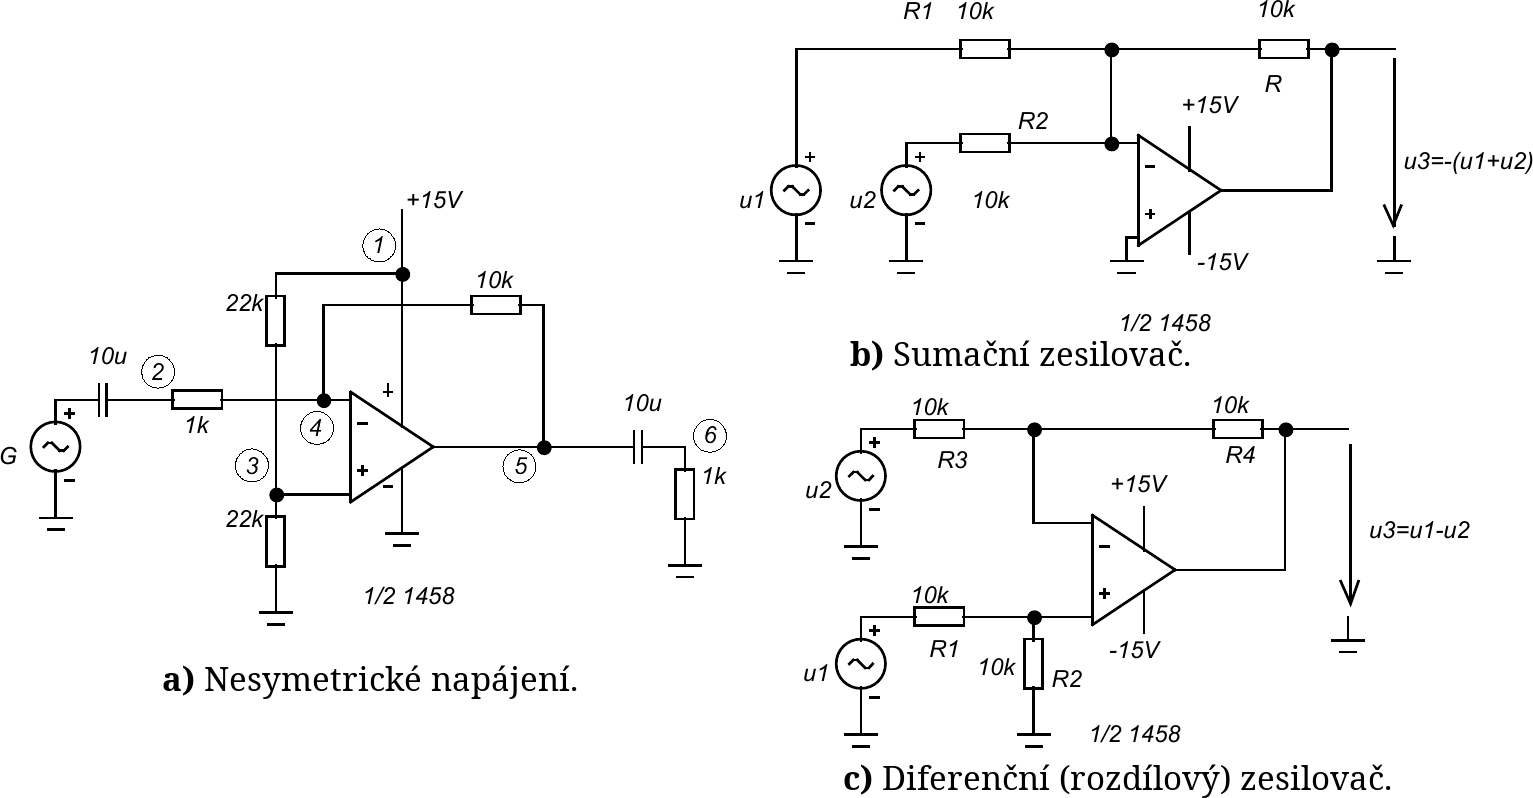
\includegraphics[width=0.8\textwidth]{schema.png}
    \centering
    \caption{Schémata zapojení -- a) AKO s jedním OZ a tranzostorovým převodníkem úrovně, b) generátor pilových kmitů}
    \label{fig:schema}
\end{figure}



\subsection{Funkce jednotlivých zapojení}

    \subsubsection{Astabilní klopný obvod}

    Základním blokem tohoto zapojení je Schmittův klopný obvod s hysterezí, ten v principu umí na výstupu zobrazovat pouze kladné a zápoorné saturační napětí. Nepřeklápí se v obou směrech stejně, ale až po překročení jisté prahové hodnoty napětí, vzniká tak hysterezní smyčka, viz Obr.~\ref{fig:hystereze-png}.

    \begin{figure}[h!]
        \centering
        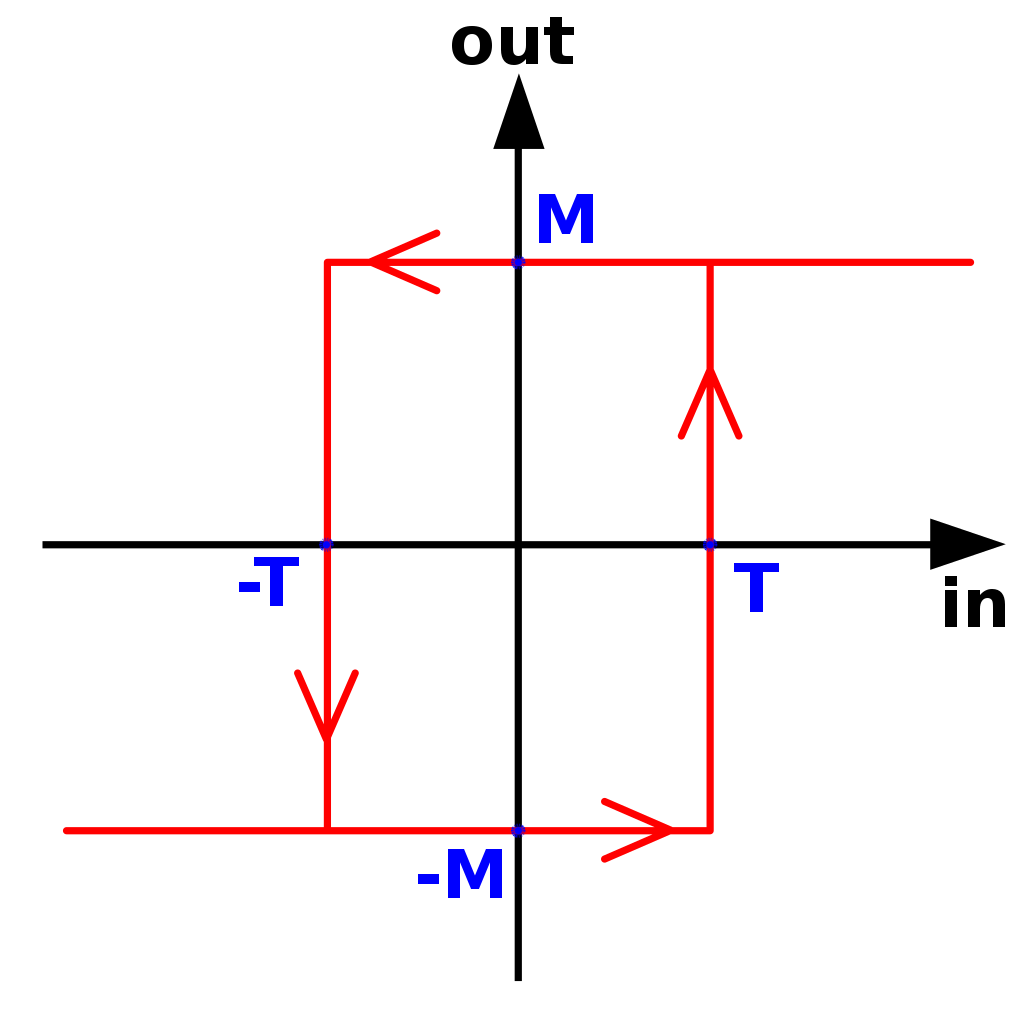
\includegraphics[width=0.5\textwidth]{hystereze.png}
        \caption{Hysterezní smyčka Schmittova klopného obvodu.}
        \label{fig:hystereze-png}
    \end{figure}
    
    Vstup tohoto obvodu je připojen k RC čánku, jehož časová konstanta nám určuje frekvenci překlápění, neboli frekvenci našich vzniklých obdélníkových pulsů, \(F=\frac{0,455}{RC}\).

    \subsubsection{Generátor pilových kmitů}

    Jako základí blok nám opět poslouží komparátor s hysterezí, ke kterému je připojen invertující integrátor, který ze vzniklých obdélníkových kmitů tvoří pilový signál.
    % Operační zesilovač s OZ má za úkol překonat nedostatky, které má zapojení pouze s diodami, které díky svému prahovému napětí nedokáží usměrňovat velmi malá napětí. 
    
    % Zapojení 1a) je jednocestný usměrňovač, kdy je vždy přes jednu diodu uzavřená záporná zpětná vazba a druhá dioda je uzavřená. Na výstupu je pak signál jednocestně usměrněný a invertovaný. 
    
    % Zapojení 1b) pak tento signál zdvojnásobí a sečte s původním vstupním signálem, ve výsledku tedy původní záporné půlvlny zůstanou a kladné po sečtení odpovídají opět záporným. Výsledkem je tedy dvoucestně usměrněný invertovaný signál. 
    % Nevýhodou tohoto zapojení je nutnost použít dva co nejshodnější odpory a k nim jeden, který odpovídá hodnotu přesně polovině, při nedodržení nebudou na výstupu půlvlny stejně velké, toto značně zdražuje zapojení. 

    % Tento problém se snaží řešit zapojení 1c), kdy pro správnou funkci stačí jedna dvojice přesných odporů \( R_2\) a \(R_3\). Záporná zpětná vazba prvního OZ je vždy uzavřena přes druhý OZ, díky diodám je ale cesta zpětné vazby jiná pro kladný a pro záporný signál, takže ve výsledku je na výstupu druhého OZ signál vždy kladný, neboli dvoucestně usměrněný.   